Qui di seguito viene riportato il codice relativo alla soluzione iniziale (non ottimizzata) del fitro FIR in questione.

\lstinputlisting[language=C++]{solutions/unoptimized/fir_unoptimized.cpp}

In particolare, si può notare come l'input, l'output e i coefficienti utilizzati risultano essere definiti rispettivamente tramite i tipi \textit{samplesType}, \textit{samplesType} e \textit{coeffsType}, cioè tutti e tre definiti come tipi di dato \textit{int} come descritto in \textit{definitions.h}. 
Bisogna specificare che l'operazione di convoluzione è stata ottenuta mediante il loop qui sopra definito. Tale operazione è data dallo shifting dei valori di input al filtro e, successivamente, dall'accumulo. Quest'ultimo è ottenuto mediante la somma, tra la corrente calcolata e la precedente accumulata, e il prodotto, tra il valore shiftato nella precedente iterazione e il coefficiente \textit{i-esimo} corrispondente.\\
Infine, il valore accumulato nella variabile \textit{accumulator} viene assegnato all'output atteso dalla procedura.\\
Effettuando la sintesi è possibile evidenziare il seguente report:\\

\begin{table}[H]
    \centering
    \begin{minipage}[t]{0.45\linewidth}
        \centering
        \begin{tabular}{|c|c|c|c|}
            \hline
            \textbf{Clock} & \textbf{Target} & \textbf{Estimated} & \textbf{Uncertainty} \\
            \hline
            ap\_clk & 10.00 & 8.510 & 1.25 \\
            \hline
        \end{tabular}
        \caption{HLS Unoptimized Solution Timing Summary (ns)}
        \label{tab:hls-unoptimized-solution-timing-summary}
    \end{minipage}
    \hfill
    \begin{minipage}[t]{0.45\linewidth}
        \centering
        \begin{tabular}{|c|c|c|c|}
            \hline
            \multicolumn{2}{|c|}{\textbf{Latency}} & \multicolumn{2}{|c|}{\textbf{Interval}} \\
            min & max & min & max \\
            \hline
            23 & 45 & 23 & 45 \\
            \hline
        \end{tabular}
        \caption{HLS Unoptimized Solution Latency Summary (clock cycles)}
        \label{tab:hls-unoptimized-solution-latency-summary}
    \end{minipage}
\end{table}

Si può notare come il periodo di clock previsto è pari a 10 ns, come impostato durante la creazione della solution in questione, mentre quello stimato è minore. Questo è dovuto al fatto che il tool stima un'incertezza (assimilabile ad un margine) che permette di calcolare il periodo di clock effettivo utilizzato dal processo di sintesi.
\begin{figure}[H]
    \centering
    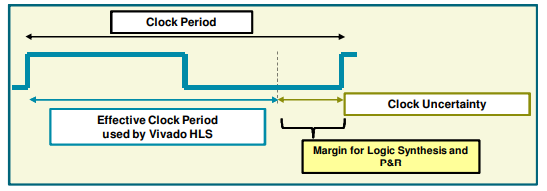
\includegraphics[width=0.5\textwidth]{solutions/unoptimized/clockperiod.png}
    \caption{HLS Clock Period from Synthesis Report}
\end{figure}

In particolare, il periodo di clock effettivo, calcolato dal tool, non deve essere considerato come parametro di progettazione ma come un margine di sicurezza previsto da HLS per il successivo place and route. Nel caso in cui si volesse operare sul periodo di clock della solution come design parameter, si dovrebbe impostare un periodo di clock differente durante la creazione della solution e poi far calcolare automaticamente l'incertezza ed il periodo del clock effettivo dallo stesso tool.

\begin{table}[H]
    \centering
    \begin{tabular}{|c|c|c|c|c|c|c|c|c|}
        \hline
        \multicolumn{1}{|c|}{Loop} & \multicolumn{2}{|c|}{\textbf{Latency}} & \multicolumn{2}{c|}{\textbf{Iteration Latency}} & \multicolumn{2}{c|}{\textbf{Initiation Interval}} & \multicolumn{1}{c|}{\textbf{Trip Count}}  \\
        Name & min & max & min & max & achieved & target &  \\
        \hline
        - loop & 22 & 44 & 2 & 4 & - & - & 11 \\
        \hline
    \end{tabular}
    \caption{HLS Unoptimized Solution Latency Loops Summary }
    \label{tab:hls-unoptimized-solution-loop-summary}
\end{table}

Considerando, invece, il loop descritto nel file sorgente, si può notare come esso presenti 11 iterazioni (corrispondenti alla capienza di processing del filtro corrispondente) e una iteration latency (IL), cioè latenza per ogni iterazione, compresa tra 2 e 4 cicli di clock. Si deduce che la latenza totale del loop in questione sia compresa tra 22 e 44 cicli di clock.
\begin{figure}[H]
    \centering
    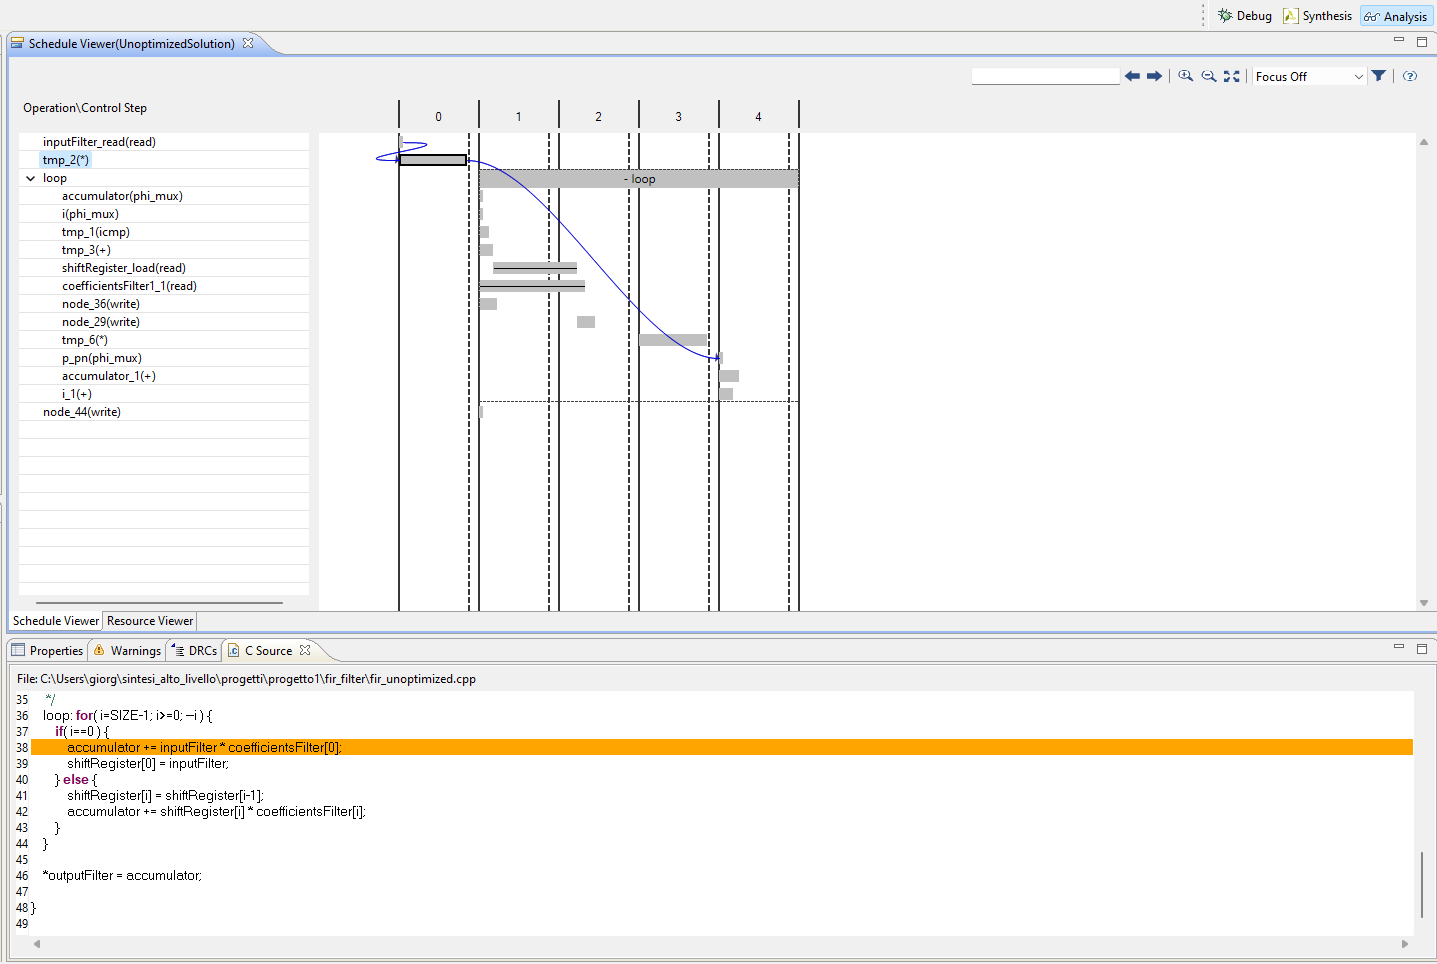
\includegraphics[width=0.7\textwidth]{solutions/unoptimized/cyclesunoptimized.png}
    \caption{HLS Unoptimized Solution If Statement Analysis}
\end{figure}

In particolare, si può notare come il ciclo di clock in più, previsto nella latenza totale dell'architettura, sia dovuto alla verifica, al calcolo e all'assegnazione in corrispondenza dell'iterazione 0 all'interno del loop. È come se l'if all'interno del ciclo for venga trattato al di fuori dello stesso loop. Questo può essere notato facendo riferimento alle operazioni svolte all'interno del loop.

Inoltre, si può notare come le operazioni di lettura previste all'interno del loop siano svolte in parallelo (come mostrato nel primo gruppo di figure allegato), mentre quelle di scrittura schedulate in differente maniera (come mostrato nel secondo gruppo di figure allegato).
\begin{figure}[H]
    \centering
    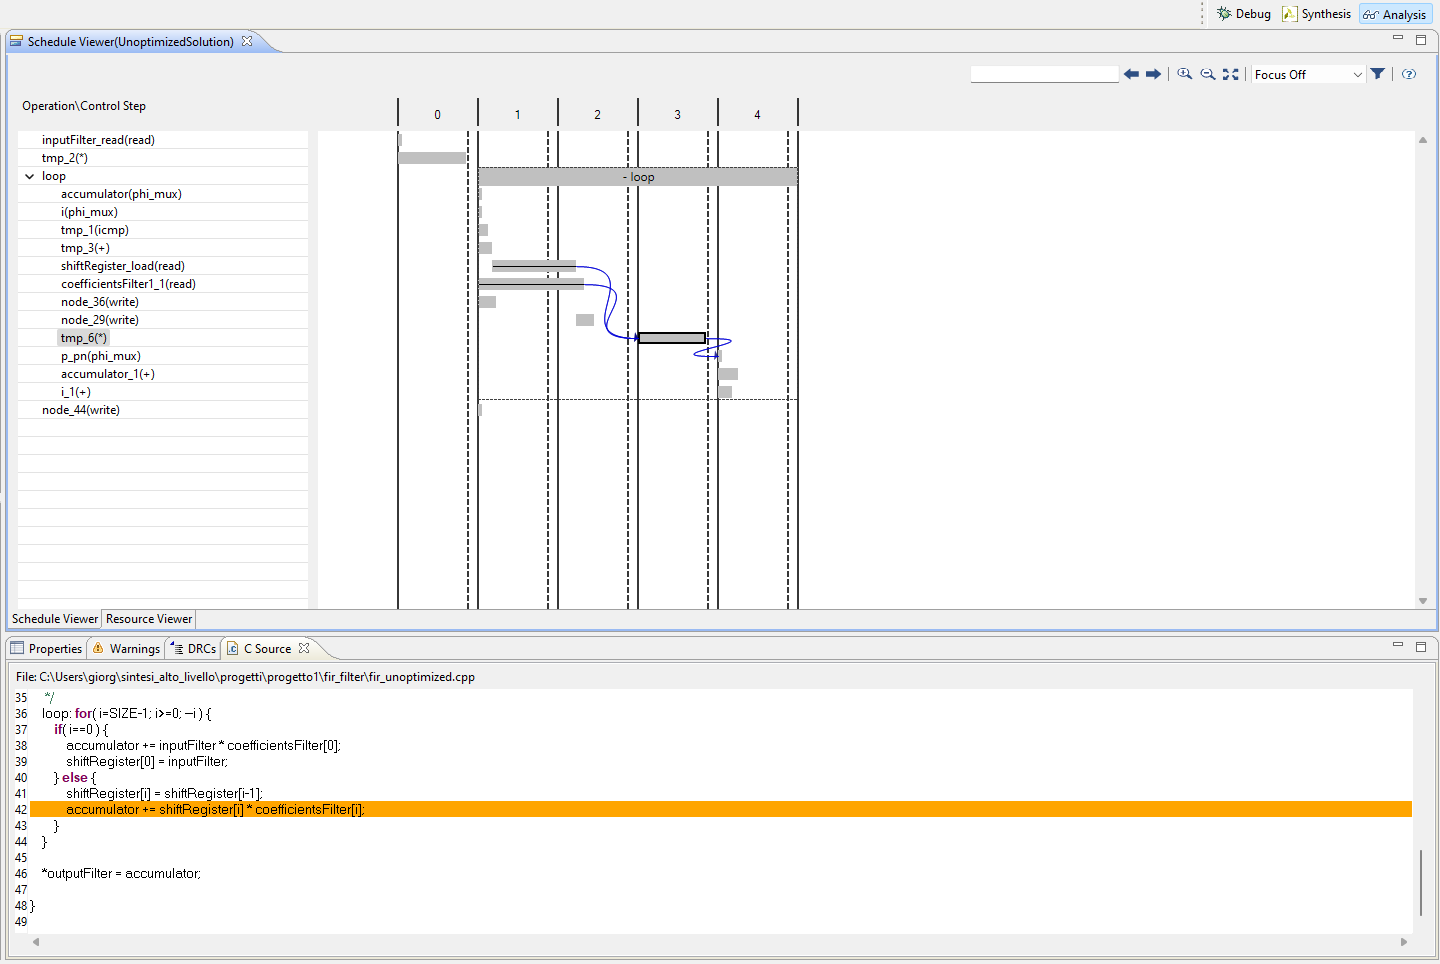
\includegraphics[width=0.7\textwidth]{solutions/unoptimized/cyclesunoptimized2.png}
    \caption{HLS Unoptimized Solution Else Statement Analysis}
\end{figure}

Infatti, si può notare come la latenza associata alle operazioni previste nelle rimanenti iterazioni del loop venga correlata alla latency associata al ciclo stesso.
\begin{figure}[H]
    \centering
    \begin{minipage}[b]{0.45\textwidth}
        \centering
        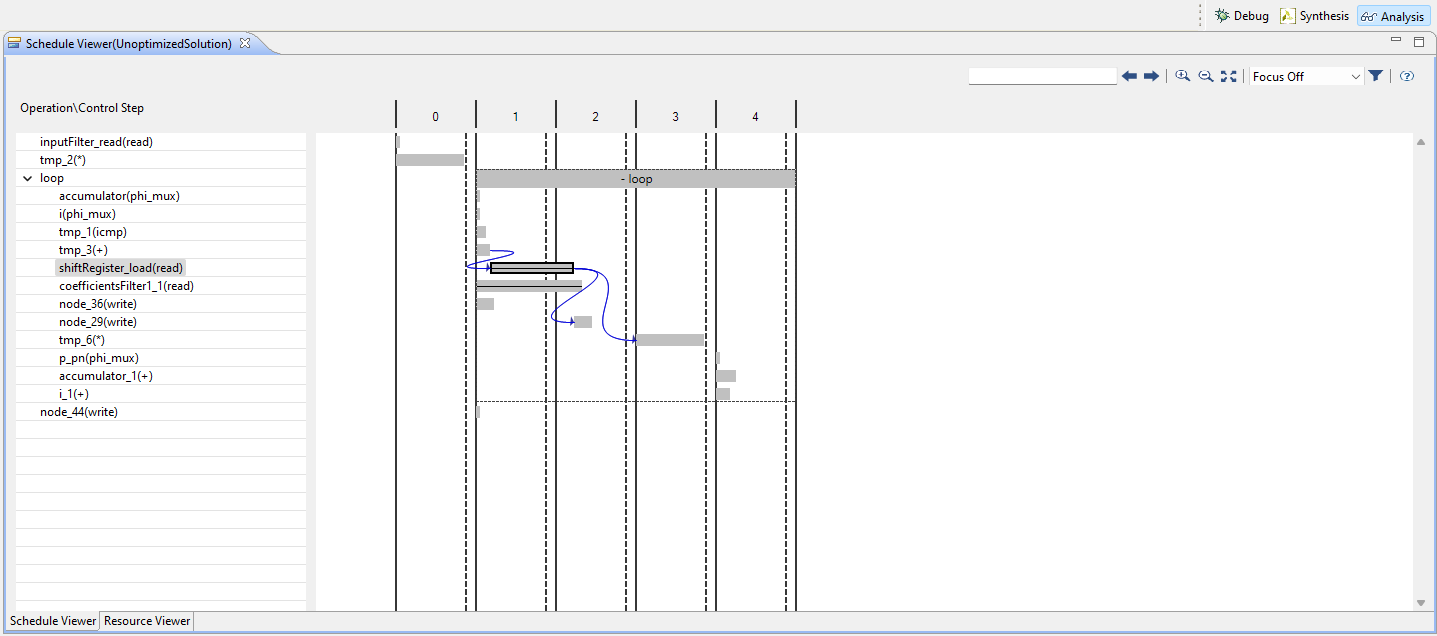
\includegraphics[width=\textwidth]{solutions/unoptimized/cyclesunoptimized3.png}
        \caption{HLS Unoptimized Solution Read Operations Analysis}
        \label{fig:left}
    \end{minipage}
    \hfill
    \begin{minipage}[b]{0.45\textwidth}
        \centering
        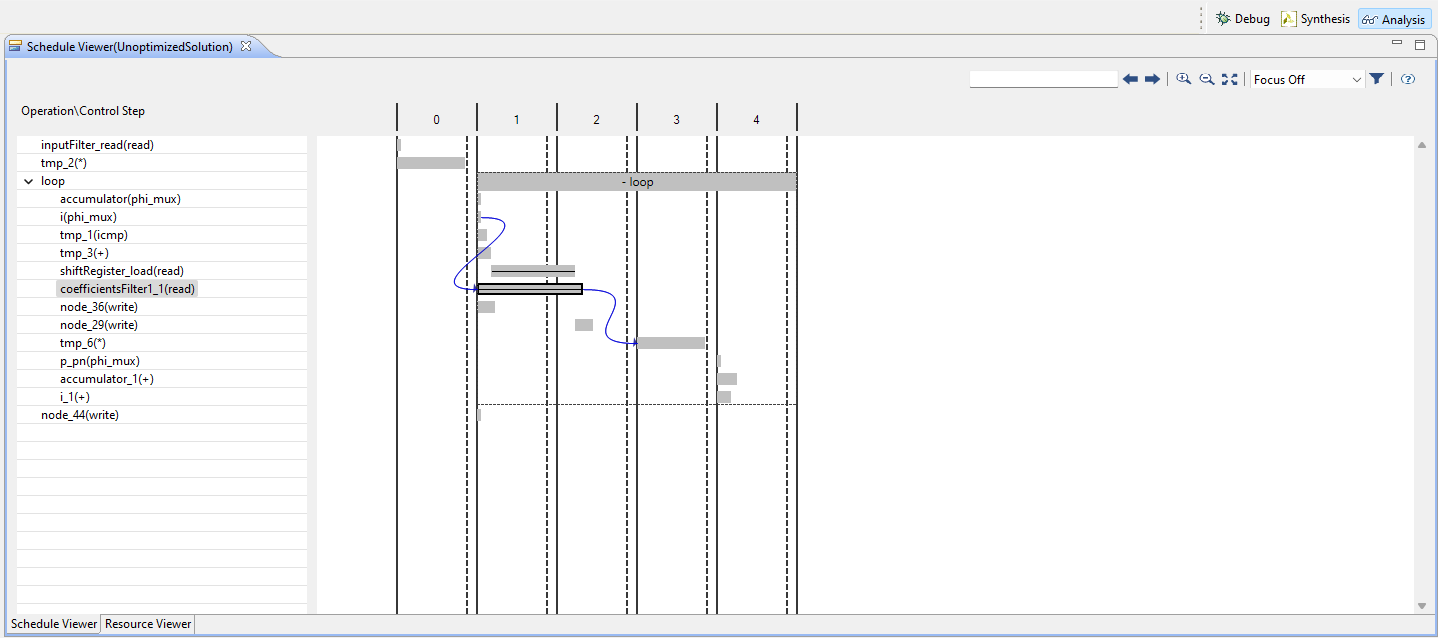
\includegraphics[width=\textwidth]{solutions/unoptimized/cyclesunoptimized4.png}
        \caption{HLS Unoptimized Solution Read Operations Analysis}
        \label{fig:right}
    \end{minipage}
\end{figure}
\begin{figure}[H]
    \centering
    \begin{minipage}[b]{0.45\textwidth}
        \centering
        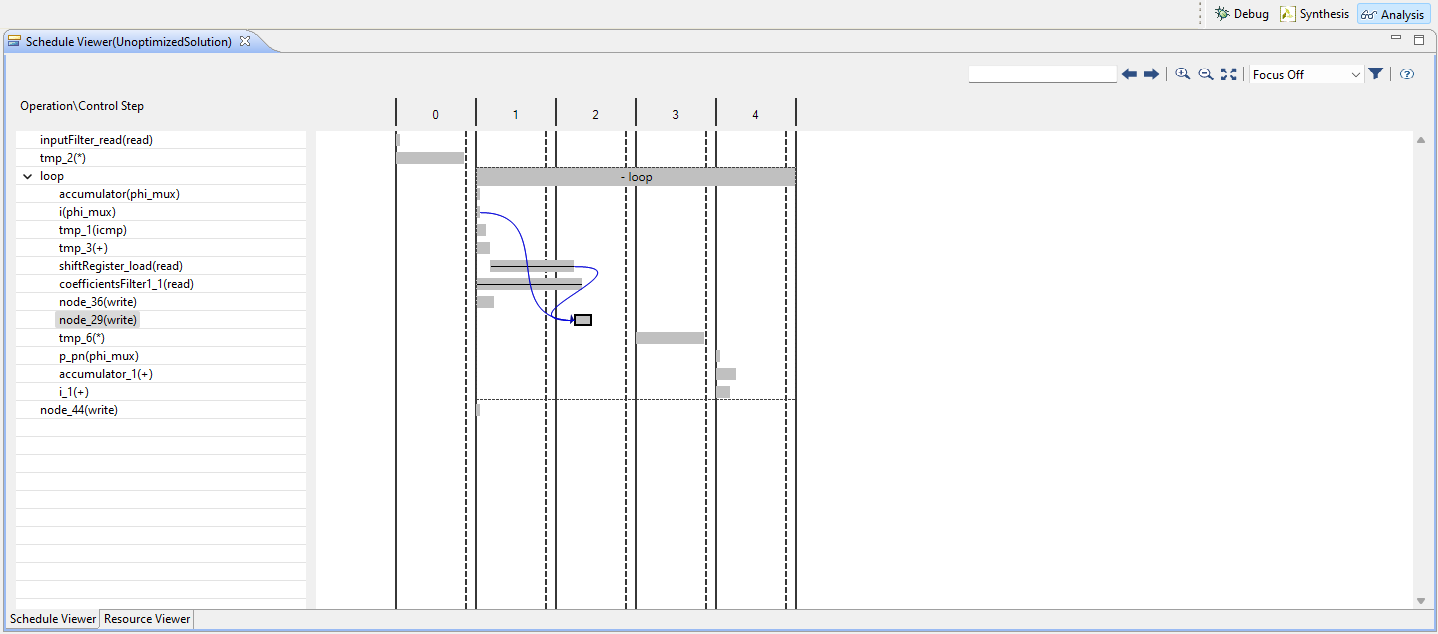
\includegraphics[width=\textwidth]{solutions/unoptimized/cyclesunoptimized5.png}
        \caption{HLS Unoptimized Solution Write Operations Analysis}
        \label{fig:left}
    \end{minipage}
    \hfill
    \begin{minipage}[b]{0.45\textwidth}
        \centering
        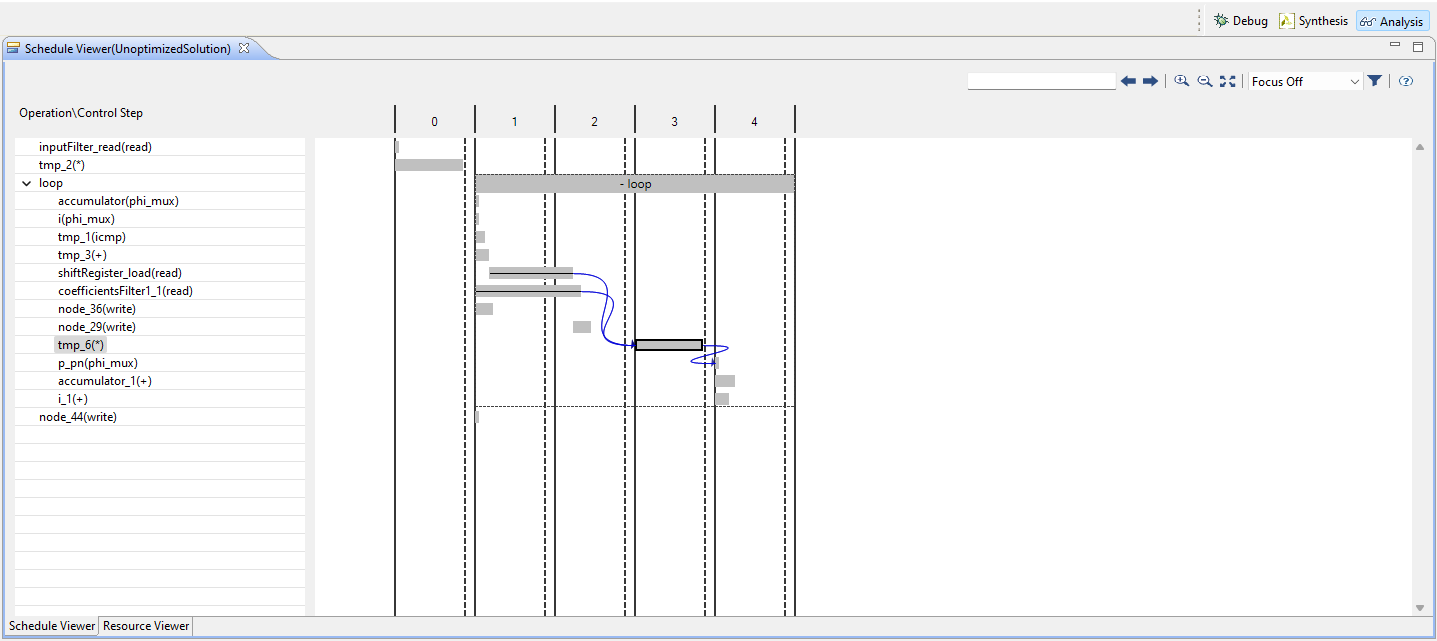
\includegraphics[width=\textwidth]{solutions/unoptimized/cyclesunoptimized6.png}
        \caption{HLS Unoptimized Solution Write Operations Analysis}
        \label{fig:right}
    \end{minipage}
\end{figure}

Qui di seguito, viene allegato l'utilizzazione delle risorse stimata dal processo di sintesi.
\begin{table}[h]
    \centering
    \begin{tabular}{|l|c|c|c|c|}
        \hline
        \textbf{Name}    & \textbf{BRAM\_18K} & \textbf{DSP48E} & \textbf{FF} & \textbf{LUT} \\ \hline
        DSP              & -                   & -               & -           & -            \\ 
        Expression       & -                   & 4               & 0           & 105          \\ 
        FIFO             & -                   & -               & -           & -            \\ 
        Instance         & -                   & -               & -           & -            \\ 
        Memory           & 0                   & -               & 74          & 8            \\ 
        Multiplexer      & -                   & -               & -           & 120          \\ 
        Register         & -                   & -               & 213         & -            \\ \hline
        \textbf{Total}   & 0                   & 4               & 287         & 233          \\ \hline
        \textbf{Available} & 280               & 220             & 106400      & 53200        \\ \hline
        \textbf{Utilization (\%)} & 0            & 1               & $\sim$0     & $\sim$0      \\ \hline
    \end{tabular}
    \caption{HLS Unoptimized Solution Utilization Estimates Summary}
    \label{tab:hls-unoptimized-solution-utilization-estimates-summary}
\end{table}

Successivamente effettuando la C/RTL Cosimulation è possibile evidenziare il seguente report:
\begin{table}[H]
    \centering
    \begin{tabular}{|c|c|c|c|c|c|c|c|}
        \hline
        \multicolumn{1}{|c|}{RTL} & \multicolumn{1}{|c|}{Status} & \multicolumn{3}{c|}{\textbf{Latency}} & \multicolumn{3}{c|}{\textbf{Interval}} \\
        &  & min & avg & max & min & avg & max \\
        \hline
        VHDL & Pass & 43 & 43 & 44 & 43 & 43 & 44 \\
        \hline
    \end{tabular}
    \caption{HLS Unoptimized Solution C/RTL Cosimulation Summary }
    \label{tab:hls-unoptimized-solution-cosimulation-summary}
\end{table}
Questa tabella mostra quanti cicli di clock sono necessari affinché venga fornito l'ingresso e l'uscita successivi.
\\

Dopodiché si può procedere con l'Export RTL.
\begin{table}[H]
    \centering
    \begin{minipage}[t]{0.45\linewidth}
        \centering
        \begin{tabular}{|l|r|}
            \hline
            \textbf{Resource} & \textbf{VHDL} \\
            \hline
            SLICE & 81 \\
            \hline
            LUT & 275 \\
            \hline
            FF & 160 \\
            \hline
            DSP & 2 \\
            \hline
            BRAM & 0 \\
            \hline
            SRL & 0 \\
            \hline
        \end{tabular}
        \caption{HLS Unoptimized Solution Export RTL Resource Usage}
        \label{tab:hls-unoptimized-solution-export-rtl-resoruce-usage}
    \end{minipage}
    \hfill
    \begin{minipage}[t]{0.45\linewidth}
        \centering
        \begin{tabular}{|l|r|}
            \hline
            \textbf{Timing} & \textbf{VHDL} \\
            \hline
            CP required & 10.000 \\
            \hline
            CP achieved post-synthesis & 5.745 \\
            \hline
            CP achieved post-implementation & 6.410 \\
            \hline
        \end{tabular}
        \caption{HLS Unoptimized Solution Export RTL Final Timing}
        \label{tab:hls-unoptimized-solution-export-rtl-final-timing}
    \end{minipage}
\end{table}
Si può notare come il numero di Flip Flop e di DSP sia diminuito rispetto a quello stimato nel report di sintesi. Questo è dovuto al fatto che, l'Export RTL non è una vera e propria implementazione ma si tratta di un processo durante il quale il tool effettua dei miglioramenti. 
\\
Successsivamente a tale fase si procede con l'importazione del'IP in Vivado. 
\lstinputlisting[language=VHDL]{solutions/unoptimized/firConvolutionUnoptimized_top.vhd}
\lstinputlisting[language=VHDL]{solutions/unoptimized/firConvolutionUnoptimized_tb.vhd}
\lstinputlisting[language=VHDL]{solutions/unoptimized/clk_constraint.xdc}
In particolare, impostando un constraint di clock pari a 10 ns (come impostato anche in HLS) e considerando un numero di ciclo di clock pari a quelli ottenuti nel report di C/RTL Cosimulation, è possibile eseguire il processo di sintesi e implementazione.
\\
\begin{table}[H]
    \centering
    \begin{tabular}{|c|c|c|c|c|c|c|}
        \hline
        \textbf{LUT} & \textbf{LUTRAM} & \textbf{FF} & \textbf{BRAM} & \textbf{DSP} & \textbf{IO} & \textbf{BUFG} \\
        \hline
        275 & 32 & 160 & 0 & 2 & 71 & 1 \\
        \hline
    \end{tabular}
    \caption{Vivado Unoptimized Solution Utilization Report [\#]}
    \label{tab:vivado-unoptimized-solution-utilization-reproot}
\end{table}

\begin{table}[H]
    \centering
    \begin{tabular}{|c|c|c|c|}
        \hline
        \textbf{Cycles} [\#] & \textbf{Clock Constraint} [ns] & \textbf{WNS} [ns] & \textbf{Maximum Clock Frequency} [Mhz] \\
        \hline
        44 & 10 & 3.654 & 157.5795777 \\
        \hline
    \end{tabular}
    \caption{Vivado Unoptimized Solution Timing Report}
    \label{tab:vivado-unoptimized-solution-timing-reproot}
\end{table}

Pertanto, dopo aver effettuato la Post-Implementation Timing Simulation e aver inserito il file \textit{.saif} all'interno dell'Implementation Power Report, è possibile analizzare con dettaglio la potenza dinamica e l'energia per singola operazione associata.

\begin{table}[H]
    \centering
    \begin{tabular}{|c|c|c|c|c|c|c|}
        \hline
        \textbf{BRAM} & \textbf{Clock Enable} & \textbf{Clocks} & \textbf{DSP} & \textbf{Logic} & \textbf{Set/Reset} [mW] & \textbf{Data} \\
        \hline
        0 & 0.454227469 & 1.215484925 & 0.335011806 & 0.921480532 & 3.57E-03 & 1.007059589 \\
        \hline
    \end{tabular}
    \caption{Vivado Unoptimized Solution Dynamic Power Report [mW]}
    \label{tab:vivado-unoptimized-solution-dynamic-power-reproot}
\end{table}

\begin{table}[H]
    \centering
    \begin{minipage}[t]{0.45\linewidth}
        \centering
        \begin{tabular}{|c|}
            \hline
            \textbf{Dynamic Total} \\
            \hline
            3.936829417 \\
            \hline
        \end{tabular}
        \caption{Vivado Unoptimized Solution Dynamic Power Report [mW]}
        \label{tab:vivado-unoptimized-solution-dynamic-power-reproot}
    \end{minipage}
    \hfill
    \centering
    \begin{minipage}[t]{0.45\linewidth}
        \centering
        \begin{tabular}{|c|}
            \hline
            \textbf{Energy Single Operation} \\
            \hline
            39.36829417 \\
            \hline
        \end{tabular}
        \caption{Vivado Unoptimized Solution Energy Single Operation Report [pJ]}
        \label{tab:vivado-unoptimized-solution-energy-single-operation-reproot}
    \end{minipage}
\end{table}

Quindi, dopo aver generato i report associati alla soluzione iniziale non ottimizzata, si può procedere con le successive soluzioni che cercheranno di migliorare diversi aspetti dell'architettura appena proposta. In particolare, nelle successive sezioni verranno commentati i risultati in termini di potenza, timing e risorse facendo riferimento alla soluzione iniziale o a quella precedente su cui sarà basata la corrente.